\documentclass{article}

\usepackage{amsmath}
\usepackage{graphicx}
\usepackage{xcolor}
\usepackage[export]{adjustbox}
\RequirePackage[margin=1in]{geometry}

\newcommand\todo[1]{\textcolor{red}{TODO: #1}}

\newcommand\animation[1]{\textcolor{blue}{ANIMATION: #1}}

\begin{document}
	
\title{Hillshade Video Script}
\author{Nathan Stouffer}
\date{}
\maketitle

\section{Intro}

\subsection{Motivation}

What I'm showing you right now is a map.
But you probably didn't need to be told that.
In fact, I would be willing to bet that you know a lot more than that.
You can probably see that this particular spot is relatively flat and that this other area is pretty steep, that this is a small gully and this is a ridgeline, and that this face is pretty rugged while this slope is not quite as technical.

You are able to get all that complex information from a pretty simple grayscale image.
In fact, I would be willing to bet that your understanding of this map is better than if I had given you the contour lines even though that is a more precise way to convey information.
Here is a side-by-side to compare.

\animation{Bring in more maps (one with just contours and another with contours/hillshade)}

This map is intentionally set up so that your brain can intuit the shape of the terrain.
Modern computers do much of this work today, but cartographers have been using versions of this technique for hundreds of years.
And many other applications use similar strategies to help convey geometric information to your brain.

The topic I'd like to discuss today is a lighting technique called hillshade.
We're going to talk about why it's such an effective method of terrain lighting and walk through the math that powers it.

\begin{center}
	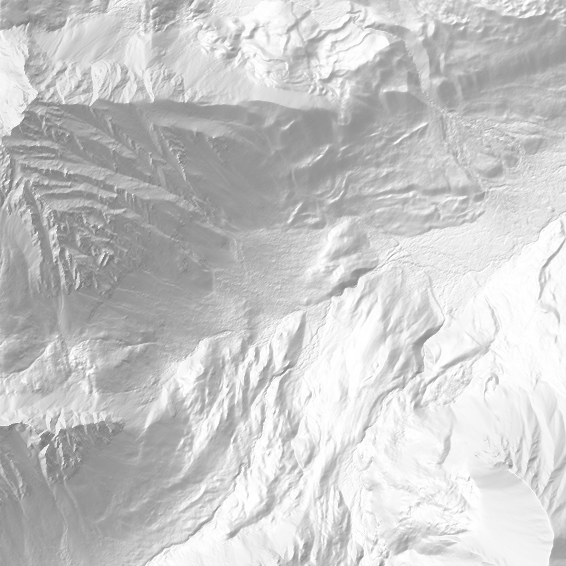
\includegraphics[width=0.5\textwidth,frame]{assets/hillshade-example.png}
\end{center}

\subsection{Directional Lighting}

We'll be discussing hillshade, but it's worth mentioning that hillshade is a very specific example of something called a directional light.
Directional lights are used all over computer graphics and are themselves just one option for how you might want to light a scene.
What I find so intriguing about directional lights is that they give you a lot of bang for your buck.
They give you quite a bit of realism for the amount of effort that you need to expend.

\animation{Fade in a graph similar to the below image.}

\begin{center}
	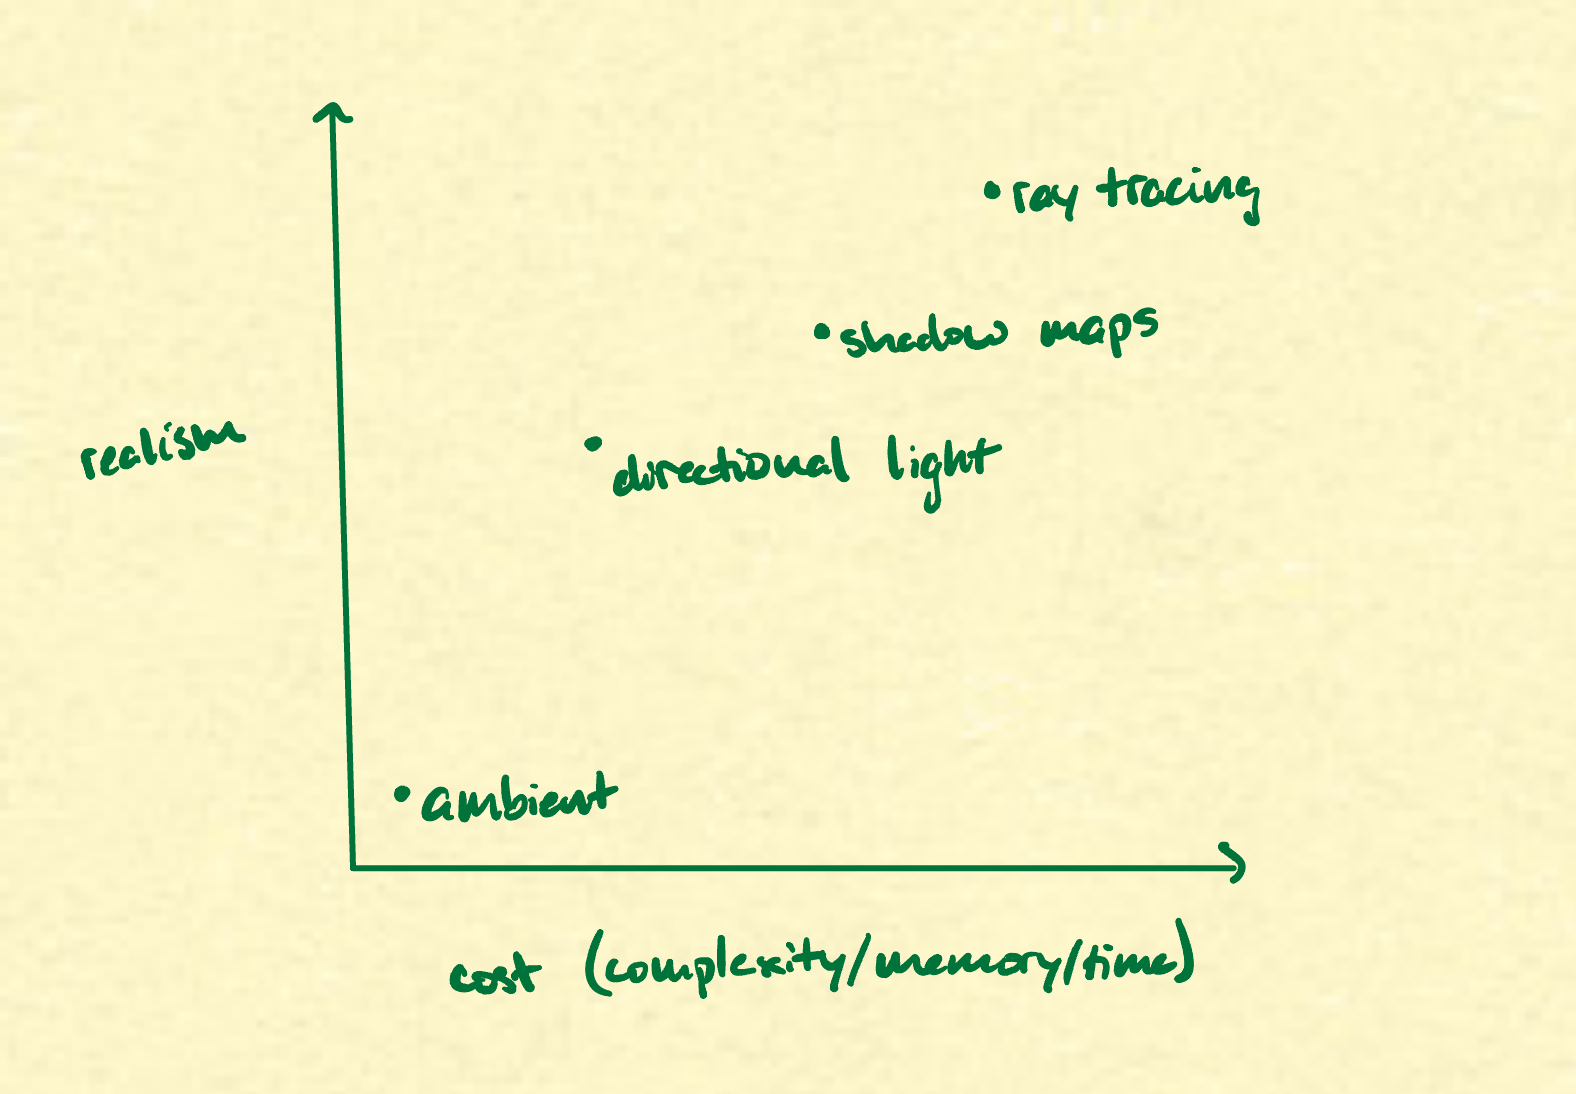
\includegraphics[width=0.65\textwidth,frame]{assets/realism.jpg}
\end{center}

If you were to represent different lighting techniques as points in the plane where the y-axis represents some notion of realism and the x-axis represents some notion of cost (maybe in terms of complexity/memory/computation time).
Then on that graph, directional lights would exist at a sweet spot where they are unreasonably effective.

So what is a directional light?
Well, a directional light is a pseudo-realistic model of how light behaves that takes a few shortcuts in the interest of simplicity.
The shortcuts come in the form of the following assumptions:

\begin{enumerate}
	
\item First, we assume that the light source is extremely far away.
If that is the case, every point in the scene has light coming from the same direction -- giving the technique its name.
You can imagine a directional light as an effect where we light up areas that face the light and shadow areas that don't.

\item The second assumption is that we ignore obstructions.
What this means is that we aren't computing true shadows -- just whether or not terrain \textit{faces} the light.
The direction is all that matters.

\end{enumerate}

The direction that the terrain faces is encoded in something called a surface normal.
The surface normal at a particular point is a vector that is orthogonal to the face of the terrain.

The light direction is given to us by configuration.
To make the math a little simpler, I am going to use the negative of the light direction.
This is the vector $l$ that points directly \textit{towards} the light source.

\animation{Show a rotating plane with a surface normal that is lit according to hillshade.}

When zoomed in on a small region of the terrain with surface normal $n$, the effect we are looking for should behave like this:
If $n$ points in the same direction as $l$, we want full-strength light.
If $l$ kind of glances off the terrain, we want half-strength light.
And if $n$ points directly opposite to $l$, we want no light at all.

\section{Hillshading}

At this point, we've covered what the effect should do, but how can we accomplish it?
What are the nuts and bolts that take this effect from a discussion of a loosely defined goal to the sequence of mathematical operations that achieve it?

\subsection{Cosine}

We can start by mathematically describing how the light strength should vary.
I'm going to gloss over the details, but the gist of the argument relies on the fact that the signed area of our rotated plane's shadow is $\cos \theta * A$ where $A$ is the area of the original plane and the sign encodes whether or not the plane faces the light source.
If an un-rotated plane gets the full light strength $S$, then a rotated plane gets strength $S * \cos \theta$.

You might notice that $\cos \theta$ can be negative.
Some directional light models ignore negative light strengths.
Hillshade takes a slightly different approach.
Remember, we want effectively light a map so that the reader can see terrain features.
When we clamp the light strength to the range $[0, 1]$, we effectively remove shading on all terrain that faces away from the light source.
Instead of clamping, it is more effective to remap the range of cosine to the interval $[0, 1]$.
This can be done by $\dfrac{1 + \cos \theta}{2}$.

\begin{center}
	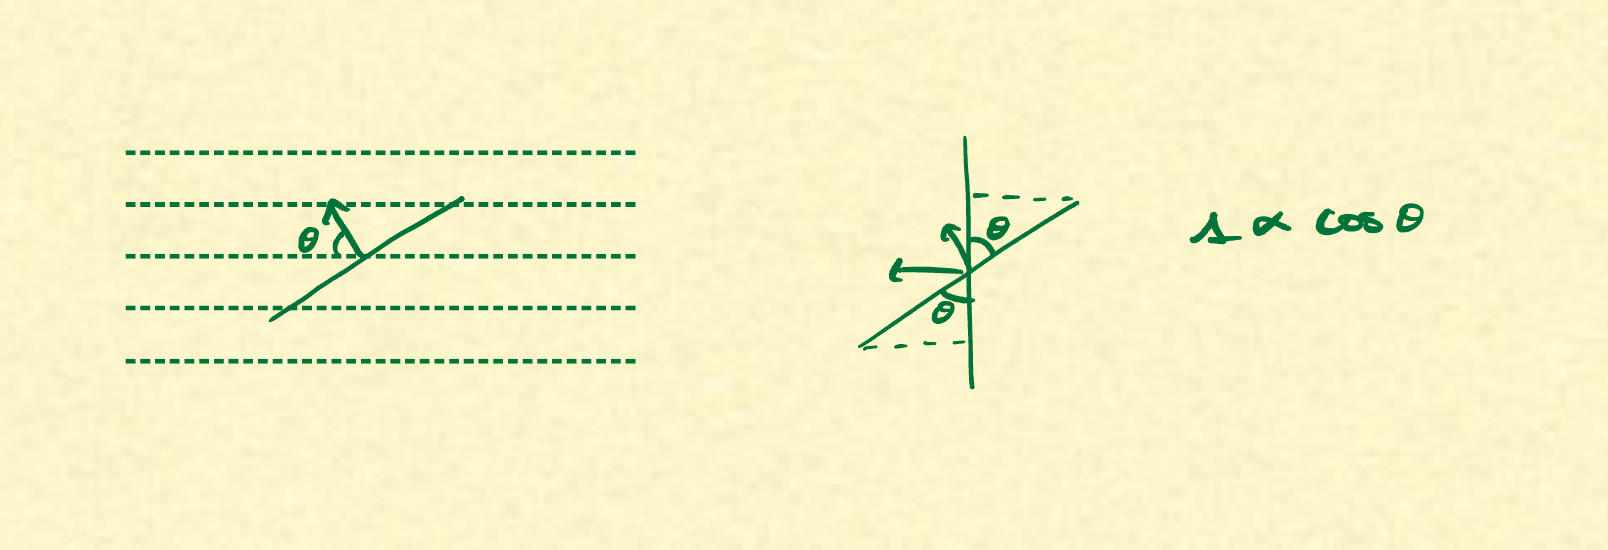
\includegraphics[width=0.75\textwidth,frame]{assets/cosine.jpg}
\end{center}

\subsection{Law of Cosines $=>$ Dot Product}

We now know that we want to vary the strength of our lighting according to $\cos \theta$.
But that doesn't really help us much because we don't know what $\theta$ is.
All we know are the vectors $l$ and $n$.
At the end of the day, those are just lists of numbers.
Sure, they have some constraints (like the fact that their length is 1).
And they also have some geometric meaning (they are directions in 3d space).
But when it comes down to it, we need to turn two lists of numbers into something as complex as the cosine function.
How are we supposed to do it?
What is the link between these two vectors and cosine?

If you were some early mathematician, at this point, you would have to start experimenting with ideas and wait for inspiration to strike.
This sort of thing takes practice and often has lots of dead ends.
It's one of those things where experience is the best teacher.

... But if I were to offer one piece of advice, I would say it's often worth constructing a triangle and using the many theorems about them to reason your way towards your goal.
Maybe it's just the types of problems that I tend to interact with, but I find triangles to be an extremely effective tool.
In this case, we are going to draw the third leg of our triangle here and use the Law of Cosines.

\begin{center}
	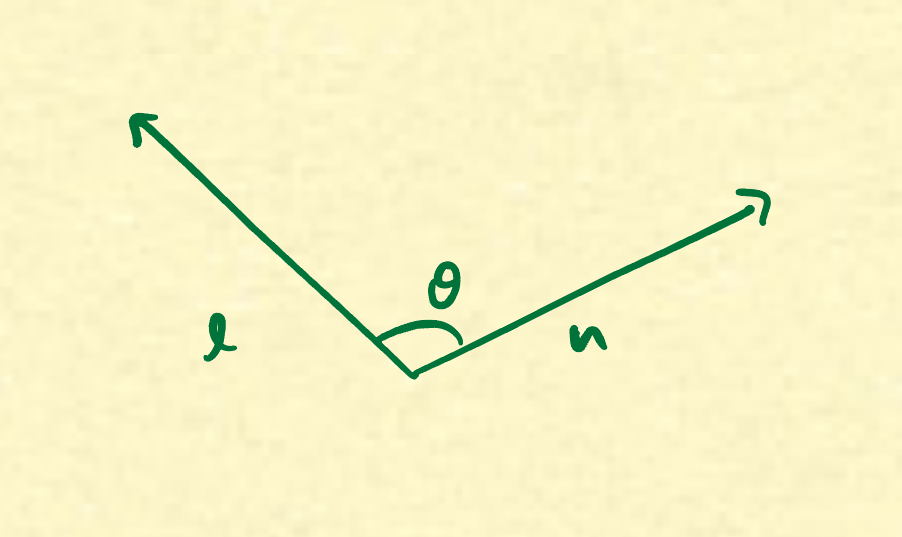
\includegraphics[width=0.3\textwidth,frame]{assets/ln.jpg}
	\hspace{0.2\textwidth}
	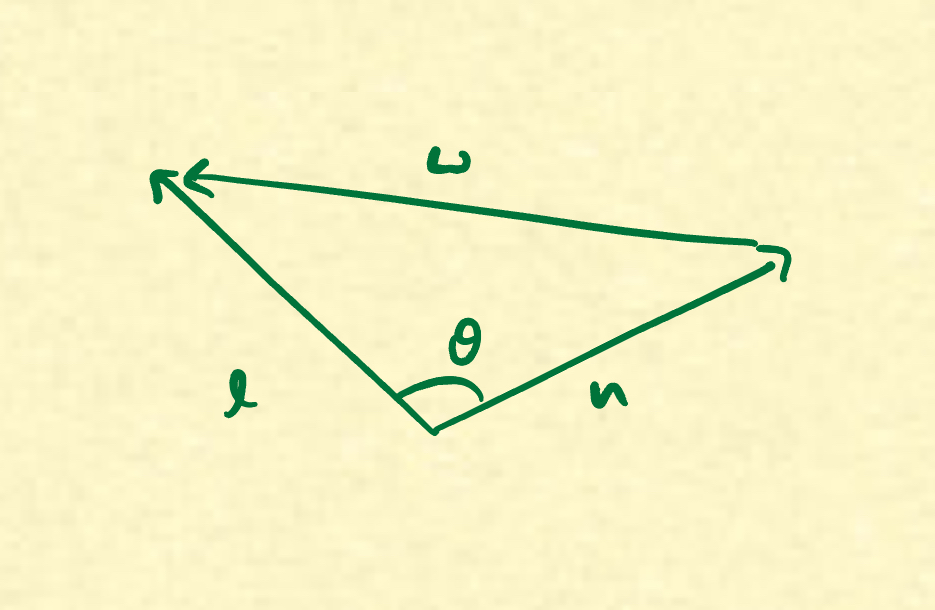
\includegraphics[width=0.2735\textwidth,frame]{assets/lnw.jpg}
\end{center}

The full Law of Cosines says that for any triangle with angles/sides labeled like so, we have $c^2 = a^2 + b^2 - 2ab \cos C$.
In our case, $a = |l|$, $b = |n|$, and $C = \theta$.
The third side is the difference between $l$ and $n$ so its length is $| l - n | ^ 2$.

\begin{align*}
|l-n|^2 = |l|^2 + |n|^2 - 2 |l| |n| \cos \theta & \quad \text{substitute from generalized LoC} \\
|l-n|^2 = 2 - 2 \cos \theta & \quad \text{since we know } |l| = |n| = 1 \\
\dfrac{2 - |l-n|^2}{2} = \cos \theta & \quad \text{simplifying}
\end{align*}

Using the Law of Cosines, we are now able to compute $\cos \theta$ just from the values of $l$ and $n$.
Those of you who are familiar with the dot product know that this can be simplified further but I am going to leave it here in the interest of accessibility.

\section{Final product}

So now we have the final product!
From earlier, we know that we want to light the terrain according to $\dfrac{1 + \cos \theta}{2}$ and we just proved that we can compute $\cos \theta$ as $\dfrac{2 - |l-n|^2}{2}$.
That's all it takes to produce the beautiful hillshade effect shown in these images.

\animation{Show a few examples.}

\section{Endnotes}

\subsection{Modified techniques}

Hillshading isn't just one thing.
It is actually a term for a family of effects that can be applied to a map.
There are a lot of variations out there.
Some examples include ambient lighting, exaggerating the normal vector, using multiple light sources, and playing around with colored lights.
You now have the mathematical framework that sits behind all of them.

\todo{Possibly mention Eduard Imhof.}

\subsection{Pseudoscopic Illusion}

In mapping, the light source for hillshade is typically placed in the northwest.
This is because most people recognize features better when the light is placed in the top left of an image, and because many maps use a north-up convention, that places the light source in the top left.

However, this can some backfire when a map with static hillshade is oriented with a south-up convention.
When that occurs, your brain might interpret everything backwards (valleys as ridges and ridges and valleys).
This is called a pseudoscopic illusion.

\animation{Show a south-up map light from the northwest and then fade in the same map (still south up) with a southeast (top left) light}.

\subsection{2D vs 3D}

I'd like to end the video by making one last comment on the simplicity of this effect: this is not a 3-dimensional map.
And I don't just mean that the screen you're viewing is 2-dimensional.
I mean that the actual model that I am rendering is 2D.

\animation{Pitch the camera}

Despite that, it is an incredibly effective method of conveying information about terrain.
I find that fascinating.

\animation{3D flythrough?}

\end{document}